
	\subsection{2.17. Сколько первых потенциалов ионизации и почему имеют молекулы: NO, O2, B2, H2O, SF6.} 
	
	\par\bigskip
	
	Потенциал ионизации молекулы.
	
	\par\smallskip
	
	Потенциал ионизации - это работа, которая требуется, чтобы
	оторвать один электрон с высшего занятого электронами уровня.
	Так, первый потенциал ионизации соответствует отрыву электрона
	с HOMO. Таким образом, потенциал ионизации молекулы равен
	взятой с обратным знаком одноэлектронной энергии
	соответствующей МО. Чем ниже расположена орбиталь, тем выше
	будет значение для первого потенциала ионизации. Чтобы говорить
	о том, что мы имеем дело с первым потенциалом ионизации,
	необходимо, чтобы в результате образовывалось ионизированное,
	но стабильное состояние системы.
	
		\begin{figure}[H]
		\centering
		{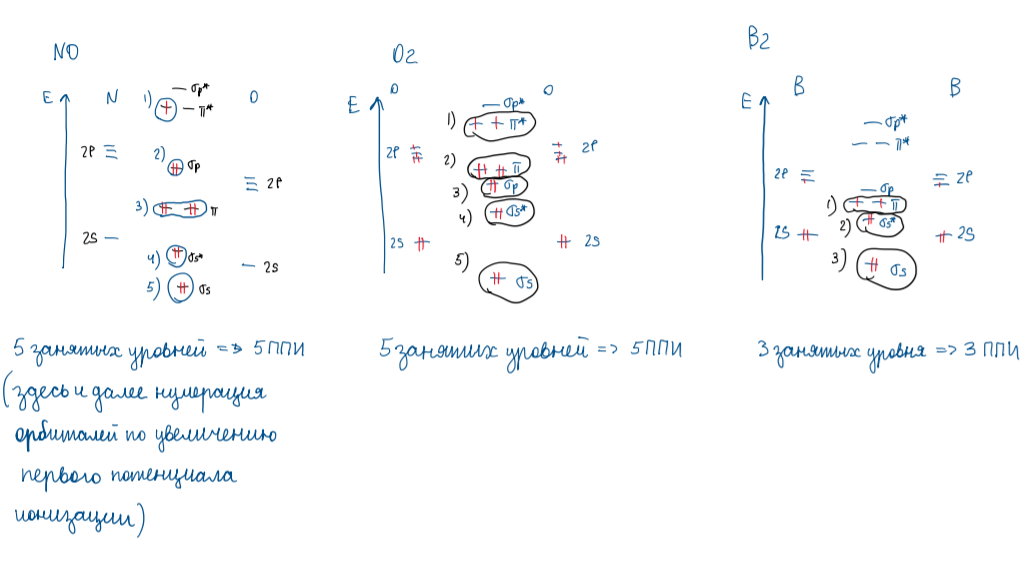
\includegraphics[scale=0.7]{49.png}}
	\end{figure}

	\begin{figure}[H]
	\centering
	{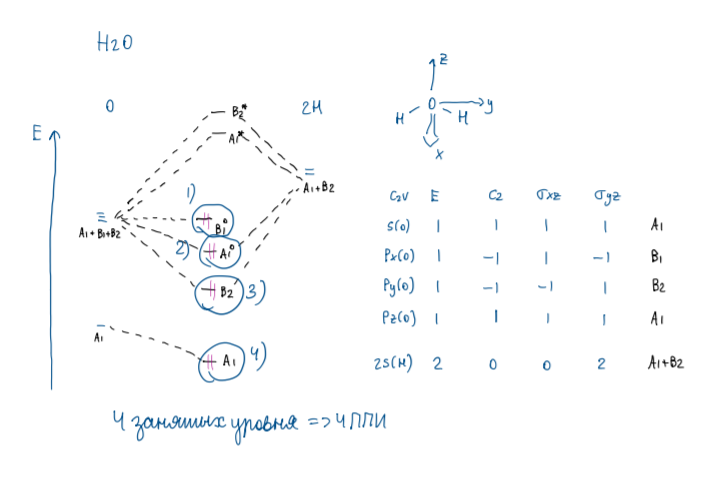
\includegraphics[scale=1]{50.png}}
\end{figure}
	
		\begin{figure}[H]
		\centering
		{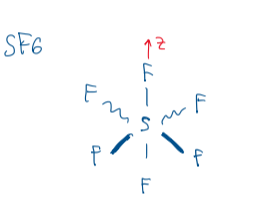
\includegraphics[scale=1]{51.png}}
	\end{figure}

В рассмотрении только p-орбитали атомов фтора, одинаковые по
симметрии с орбиталями атома серы: s-орбитали атомов фтора располагаются настолько
низко по энергии, что их можно считать
несвязывающими. При ионизации с них порядок связи
в молекуле не изменится, однако система уже не будет
стабильной, поэтому этот уровень энергии нельзя
считать одним из первых потенциалов ионизации.

\par\smallskip


На полной диаграмме с рассмотрением всех pорбиталей атомов фтора мы бы наблюдали большое
количество несвязывающих орбиталей, как раз от них.
Однако они не участвуют в образовании химической
связи, ионизация с этих орбиталей не приведет к
ослаблению связи, поэтому это тоже не ПИ.

\par\smallskip

Про t1u (несв.) под цифрой 1): пусть мы и считаем
данную орбиталь несвязывающей, всё же она хоть както перекрывается с орбиталями той же симметрии.
Экспериментально можно установить ее энергетическое
положение, возможно, она будет чуть ниже исходного
уровня, но это неважно, потому что сам факт участия в
перекрывании позволяет заключить о том, что этот
уровень энергии будет одним из ПИ.

\begin{figure}[H]
	\centering
	{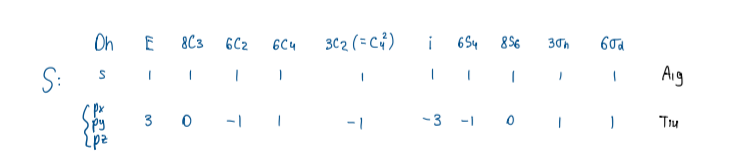
\includegraphics[scale=1]{52.png}}
\end{figure}

\begin{figure}[H]
	\centering
	{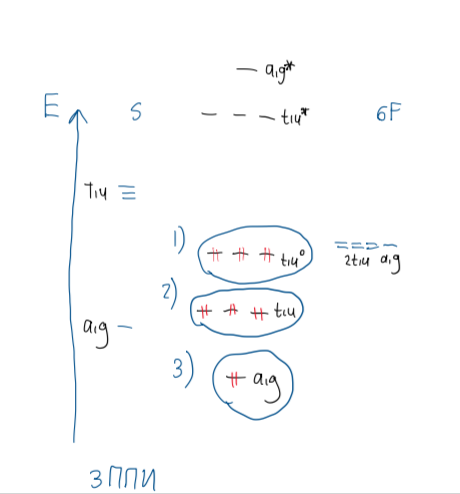
\includegraphics[scale=1]{53.png}}
\end{figure}